\chapter{Zentrales Collectorsystem}
\chapterauthor{Jannik Schäfer}



\section{Problemstellung}
    Im Gesamtsystem soll es möglich sein, sich als Nutzer einzuloggen und individuelle Daten im System zu hinterlegen.
    Dazu müssen wir ein System bereitstellen, über das sich ein Nutzer im System registrieren und anmelden kann und alle relevanten Nutzerdaten gespeichert werden.
    
    Da es sich hierbei um eine nach außen sichtbare, oberflächenlose Schnittstelle handelt, muss das System eine REST-Schnittstelle bereitstellen, welche nicht nur das Erstellen und Abfragen von Daten erlaubt, sondern auch das Authentifizeren von einzelnen Anfragen an das System. Darüber hinaus muss das System mit den anderen Diensten der Microsverice-Architektur kommunizieren um Anfragen von außen im Gesamtsystem zu verarbeiten.
    
    Zudem muss das Collectorsystem eine Möglichkeit bereitstellen beliebige Web-Inhalte im elastifeed-System zu speichern. Dafür muss eine Oberfläche bereitgestellt werden, über das ein Nutzer Inhalte im System hinterlegen kann.

\section{Laravel}
    Als Basis für das Collectorsystem verwenden wir Laravel.
    
    Laravel ist ein freies, sehr weit verbreitetes PHP-Framework, welches nach dem MVC Architekturmuster aufgebaut ist. Es wurde 2011 veröffentlicht und unterstützt ein großes Ökosystem von zusätzlichen Modulen und Komponenten, welche eine zukünftige Erweiterung des Systems stark vereinfachen. Das Laravel-Framework wird mit einer großen Menge an Modulen mitgeliefert, die bei Bedarf im System genutzt werden können.
    
    
    \subsection{Composer}
        Laravel setzt zur Verwaltung von externen Abhängigkeiten auf Composer. Composer ist eine Paketverwaltung für die Programmiersprache PHP und wird über die Commandozeile ausgeführt. Die Abhängigkeiten der Software werden mit \texttt{composer install} installiert und in einem projektspezfiscihen \texttt{/vedor} Ordner gespeichert. Weitere Abhängigkeiten können mittels \texttt{composer require username/packageName} von Packagist, dem globalen PHP Package Repository installiert werden. Informationen über die Abhängigkeiten werden in einer \texttt{composer.json} festgehalten, wo ebefalls Informationen über Namensräume, die Systemumgebung und das Projekt selbst enthalten sind. 
        
        \begin{lstlisting}[caption={Ausschnitt composer.json für das Collector-System}]
{
    "name": "laravel/laravel",
    "type": "project",
    "description": "The Laravel Framework.",
    "keywords": [
        "framework",
        "laravel"
    ],
    "license": "MIT",
    "require": {
        "php": "^7.1.3",
        "fideloper/proxy": "^4.0",
        "guzzlehttp/guzzle": "^6.3",
        "laracasts/utilities": "^3.0",
        "laravel/framework": "5.8.*",
        "laravel/passport": "^7.2",
        "laravel/tinker": "^1.0",
        "ext-json": "*"
    },
    "require-dev": {
        "beyondcode/laravel-dump-server": "^1.0",
        "filp/whoops": "^2.0",
        "fzaninotto/faker": "^1.4",
        "mockery/mockery": "^1.0",
        "nunomaduro/collision": "^3.0",
        "phpunit/phpunit": "^7.5"
    },
    
    ...
    
}
     \end{lstlisting}
     
     Im Collector-System wurde neben den Laravel spezifischen Abhängigkeiten noch folgende zusätzliche Pakete installiert:
        
        \begin{itemize}
            \item Guzzle: Bibliothek um HTTP-Requests mit PHP zu vereinfachen
            \item Passport: Bibliothek zum Ausstellen von JSON Web Tokens
        \end{itemize}
    
    \subsection{.env Umgebungsdatei}
        Die \texttt{.env} Umgebungsdatei, enthält Variabeln, welche für die Systemumgebung spezifisch festgelegt sind. Im Collector-System werden dabei insbesondere die Datenbankverbindung und ein Link zum \texttt{es-pusher} hinterlegt.
        
    \subsection{Artisan}
        Laravel wird mit einem Command-Line Tool namens Artisan mitgeliefert. Mit diesem Tool ist es möglich, das System zu installieren, zu erweitern und zu testen. Im Collector-System werden mittels Artisan die Sicherheits-Keys generiert, welche zur Authentifizierung benötigt werden und das Datenbankschema wird für die Nutzung des Systems vorbereitet.
        
        
        \begin{lstlisting}[caption={Installationsprozess mit Artisan und Composer}]
composer install
php artisan key:generate
php artisan migrate
php artisan passport:install
        \end{lstlisting}

\section{Datentypen}
    Das Zentrale Collectorsystem verwaltet Nutzer und die damit verbundenen Daten.
    Datenstrukturen werden in Laravel durch das sogenannte Eloquent ORM (Object-Relational Mapping) abstrahiert. Bei Bedarf wird dabei eine Datenbank-Tabelle im PHP-Code durch ein \texttt{Model} repräsentiert, welches genutzt werden kann um die realen Daten in der Datenbank abfzufragen oder zu manipulieren.
    
    Das Collector-System besitzt drei große Datentypen, welche mit dem Eloquent ORM im System verwendet werden.
    
    \begin{center}
        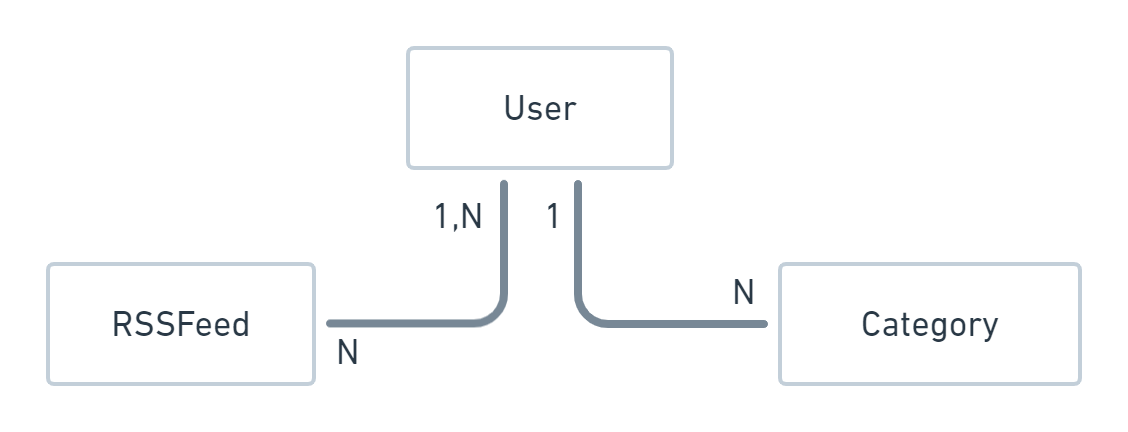
\includegraphics[width=\textwidth]{images/collector-erm.png}
        \caption{Entity-Relationship-Modell des Collector-Systems}
    \end{center}
    
    \subsection{User}
        Ein Nutzer besteht aus einer ID, einem Namen, einer einzigartigen E-Mail Adresse und einem Passwort-Hash. Darüber hinaus werden weitere Meta-Informationen mit dem Nutzer gespeichert, welche dazu dienen, die Schnittstellen-Autentifzierung zu ermöglichen.
        
        Ein User bestitzt null oder beliebig viele Kategorien und ist mit null oder beliebig vielen RSS-Feeds verbunden.
    \subsection{Kategorie}
        Eine Kategorie gruppiert eine Menge von gespeicherten Seiten. Sie besteht aus einer ID, einem Namen und Meta-Informationen im JSON-Format, welche bei Erweiterung des System mit zusätzlichen Informationen befüllt werden können.
        
    \subsection{RSS-Feed}
        Ein RSS-Feed ist ein Link zu einem realen Web-RSS-Feed. Er besteht aus einer ID, einem Link und dessen einzigartigen Hash-Wert. Ein RSS-Feed kann von einem oder mehreren Nutzern abboniert werden und ein Nutzer kann null oder beliebig viele RSS-Feeds abbonieren.
    

\section{REST-Schnittstelle}

    Im Laravel-System werden Endpunkte der Schnittstelle als Route über die \texttt{routes/api.php} definiert. Alle Anfragen an das System, welche nicht von einem Browser ausgehen werden hier aufgelöst.
    
    Eine Routendefinition besteht aus dem Pfad und einem Controller, welcher mit einer bestimmten Methode die Anfrage beantworten soll. Der Pfad kann dabei beliebig viele Platzhalter enthalten, was dynamische Routen ermöglicht. Nach diesem Prinzip wurden für alle Datentypen die nötigen REST-Endpunkte aufgebaut.
    
    Im folgenden sehen Sie ein Beispiel einer Routendefinition, bei der ein \texttt{DELETE}-Request auf \texttt{/feeds/{id}} die \texttt{removeFeeed} Methode des \texttt{app/Http/Controllers/API/FeedController}-Controllers aufruft. Der Platzhalter \texttt{{id}} ist hier in seiner Form auf einen numerischen Wert mit mindestens einem Zeichen festgelegt.

    \begin{lstlisting}
Route::delete('/feeds/{id}', 'API\FeedController@removeFeed')->where('id', '[0-9]+');
    \end{lstlisting}
    
    \subsection{Authentifizierung mittels JWT}
        Einige dieser Routen sind nur für registrierte Nutzer erreichbar. Darum werden diese durch eine Middleware, welche die Existenz und Korrektheit eines JSON Web Token prüft, geschützt. 
        
        \begin{center}
            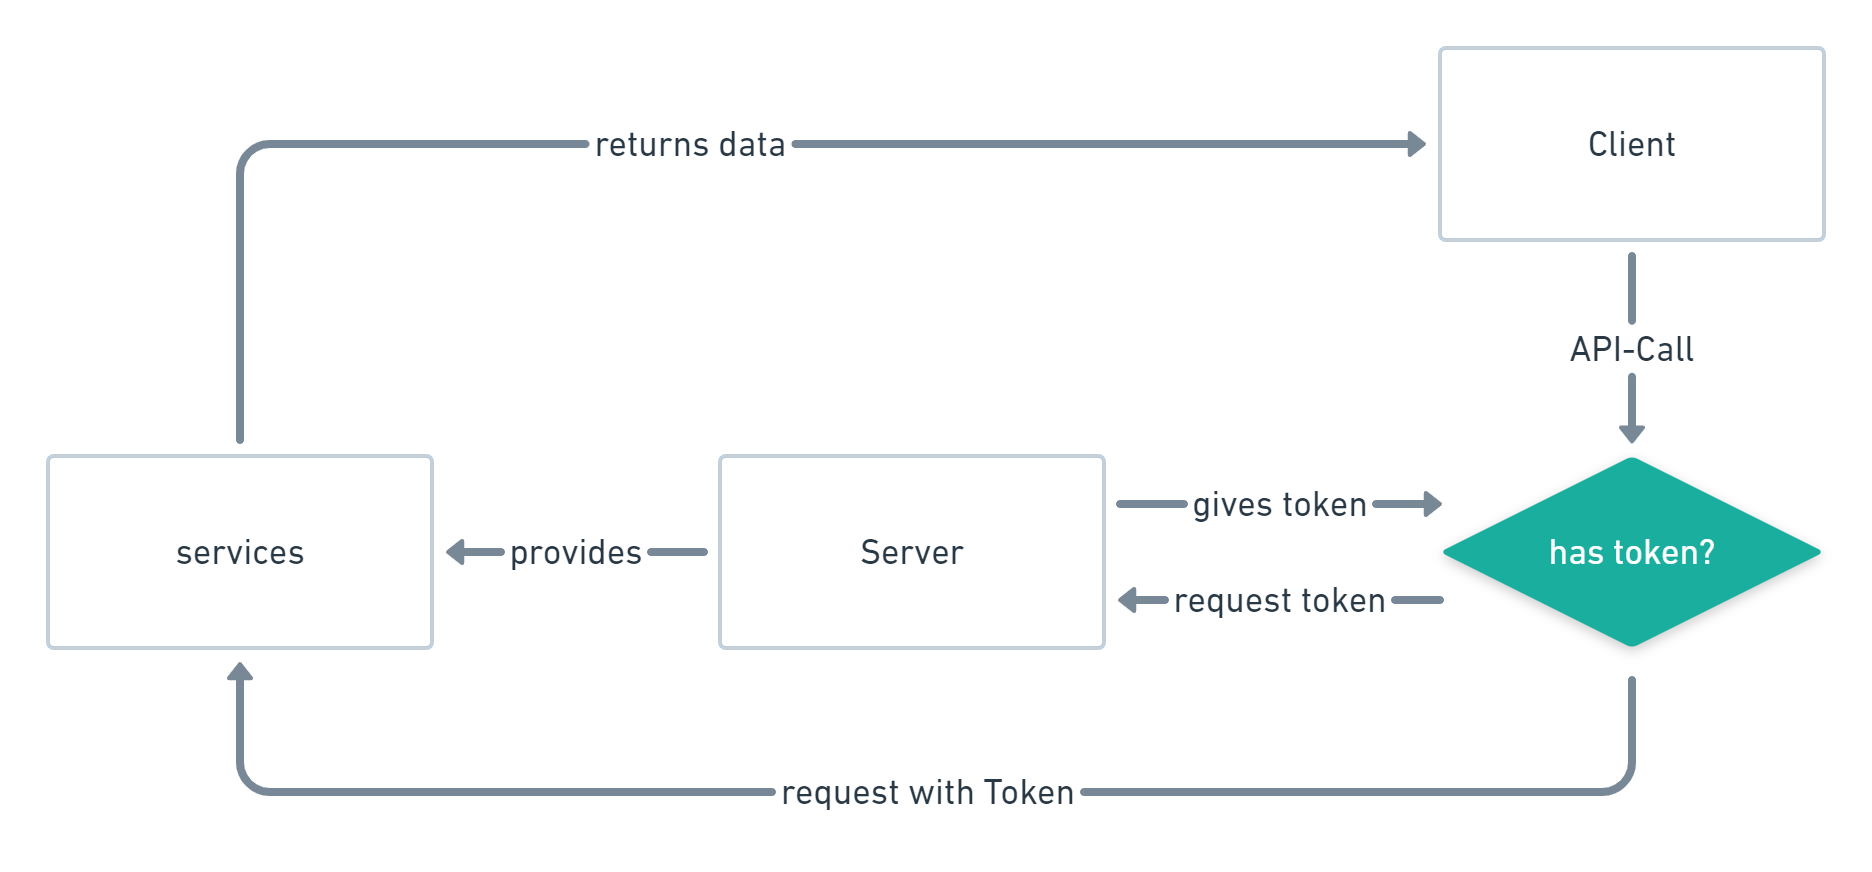
\includegraphics[width=\textwidth]{images/collector-jwt-auth-process.png}
            \caption{Schematischer Ablauf der Authentifizierungs-Middleware}
        \end{center}
        
        JSON Web Tokens (JWT) wurden mit der RFC 7519 international standartisiert und sind ein einmalig generierte Token, welches, nach Ausstellung für viele Anfragen an eine Schnittstelle, genutzt werden können, um den Nutzer zu identifizieren und autorisieren. Im Gegensatzt zur herkömlichen Name, Passwort Authentifizierung muss zwischen den einzelnen Anfragen nur das Token und nicht ein Passwort im Klartext zwischengespeichert werden.

        Im Collector-System wird das JWT im \texttt{/v1/login}-Endpunkt ausgestellt, wenn Benutzername und Passwort korrekt sind und gewährt Zugriff auf alle Nutzerspezifischen Endpunkte der REST-Schnittstelle. Voraussetzung ist dessen Präsenz im Authorization Header nach dem Bearer Schema (\texttt{Bearer: <token>}) bei jeder Anfrage.
        
        \subsubsection{Aufbau}
        Ein JSON-Web Token besteht aus folgenden Teilen, welche jeweils im JSON-Format dargestellt sind.
        \begin{itemize}
            \item Header: Enthält Metainformationen zum Token und Informationen zum verwendeten Hash-Algorithmus
            \item Inhalt: Im Token gespeicherte Informationen mit Steuerungsbefehle zur Gültigkeit, Ausstelungszeitpunkt und mehr
            \item Signatur: Header, Inhalt und ein 256 bit Key werden gemeinsam mit dem im Header definiertem Algorithmus gehasht. Die Signatur wird dazu genutzt das Token zu verifizieren.
        \end{itemize}
        
        Alle Teile des JTW werden mittels Base64URL Encode kodiert und anschließend punktsepariert zum finalen Token zusammengefügt.
        
        \begin{center}
            \textbf{Exemplarisches JWT nach Erzeugung} \\
            \texttt{eyJhbGciOiJIUzI1NiIsInR5cCI6I \\
            ODkpXVCJ9.eyJzdWIiOiIxMjM0NTY3 \\
            wikwIiwibmFtZSI6IkpvaG4gRG9lIi \\
            nJaWF0IjoxNTE2MjM5MDIyfQ.vp1xm \\
            -QE406Ay0IrTvAQ8bejQQh085lLa6u \\
            dgi2lk}
        \end{center}
        
    \subsection{Endpunkte}
        
        \subsubsection{RSS-Feeds}
            Über das Collector-System ist es möglich alle Feeds vom eingeloggten User abzurufen, neue Feeds zu abbonieren und zu Feeds zu deabbonieren.
        
            \begin{lstlisting}
Route::get('/feeds', 'API\FeedController@getAll');
Route::post('/feeds', 'API\FeedController@insertNew');
Route::delete('/feeds/{id}', 'API\FeedController@removeFeed')
    ->where('id', '[0-9]+');
            \end{lstlisting}
        
        \subsubsection{Kategorien}
            Über das Collector-System ist es möglich alle Kategorien vom eingeloggten User abzrufen, neue Kategorien zu erstellen und bestehende Kategorien zu löschen.
        
            \begin{lstlisting}
Route::get('/categories', 'API\CategoryController@getAll');
Route::post('/categories', 'API\CategoryController@insertNew');
Route::delete('/categories/{id}', 'API\CategoryController@removeCategory')
    ->where('id', '[0-9]+');
            \end{lstlisting}
        
        \subsubsection{Seiten}
            Das Collector-System stellt einen Endpunkt bereit, über den eine Webseite dem Nutzer-Index hinzugefügt werden kann.
            \begin{lstlisting}
Route::post('/page', 'API\PageController@pushNew');
            \end{lstlisting}

        \subsubsection{User}
            Neue Nutzer können im \texttt{/v1/register}-Endpunkt angelegt werden. Ein registrierter Nutzer kann sich im \texttt{/v1/login}-Endpunkt ein Token ausstellen lassen und anschließend seine Eigenen Informationen im \texttt{/v1/me}-Endpunkt abfragen.
            
            \begin{lstlisting}
Route::post('/login', 'API\UserAuthController@login');
Route::post('/register', 'API\UserAuthController@register');
Route::group(['middleware' => 'auth:api'], function (){
    Route::get('/me', 'API\UserAuthController@getCurrentUser');
});
            \end{lstlisting}


\section{Speichern von Seiten}
    Eine weitere Anforderung am Projekt war es, dass ein Nutzer, während er im Browser eine Seite betrachtet, diese sofort im elastifeed-System abspeichern kann. Es muss also möglich sein, aus dem Browser, ohne das Fenster oder den Tab zu wechseln eine Webseite oder einen Feed im System abspeichern zu können. Mit einem Browser-Plugin kann diese Funktion zwar realisiert werden, doch es müsste für alle gängigen Browser ein seperates Plugin entwickelt werden. Je nach Browser unterscheiden sich technische Voraussetzungen und Möglichkeiten, was die Bereitstellung eines einheitlichem und zukunftssicherem Systems erschwert. Um den Aufwand klein zu halten, stellen wir ein Bookmarklet bereit, welches den Nutzer in eine Web-Application, den Client-Pusher, führt, wo die Seite final im System gespeichert werden kann.
    
    Da das Collector-System als öffentliche Schnittstelle bereits von außen erreichbar ist, wird das Bookmarklet und der Client-Pusher über das Laravel-System bereitgestellt.
    
    \subsection{Bookmarklet}
        Ein Bookmarklet ist ein Link, welcher auf Klick JavaScript-Code im aktuellem Browser-Tab ausführt. Dieser Link kann ganz einfach mittels Drag-and-Drop in die Lesezeichen-Leiste jedes Browser gezogen werden, womit der Nutzer von überall auf den JavaScript-Code zugreifen kann.
        
        Das elastifeed Bookmarklet merkt sich lediglich die aktuelle URL und leitet anschließend in das Collector-System um, wo der Client-Pusher dafür zuständig ist, das Speichern der Seite im elastifeed-System auszuführen.
        
        \begin{lstlisting}[caption=HTML Aufbau eines Bookmarklet]
<a href="javascript:(function(){ alert('hello world'); })();">
hello world bookmarklet
</a>
        \end{lstlisting}

    \subsection{Client-Pusher}
        Der Client-Pusher ist eine eigenständige Web-Applikation basierend auf dem weit verbreitetem JavaScript-Framework React. React ist darauf spezialisiert dynamische Nutzeroberflächen im Browser darzustellen und wir vom Collector-System bereitgestellt. Der Client-Pusher kommuniziert dabei zur Laufzeit mit der REST-Schnittstelle des Collector-Systems um die Seiten- oder RSS-Feed-Daten vorzubereiten und schließlich im System zu speichern.

        Abhängig vom zu speicherndem Inhalt, kann der Nutzer individuelle Metadaten hinterlegen und anschließend den finalen Speichervorgang bestätigen.

        \begin{center}
            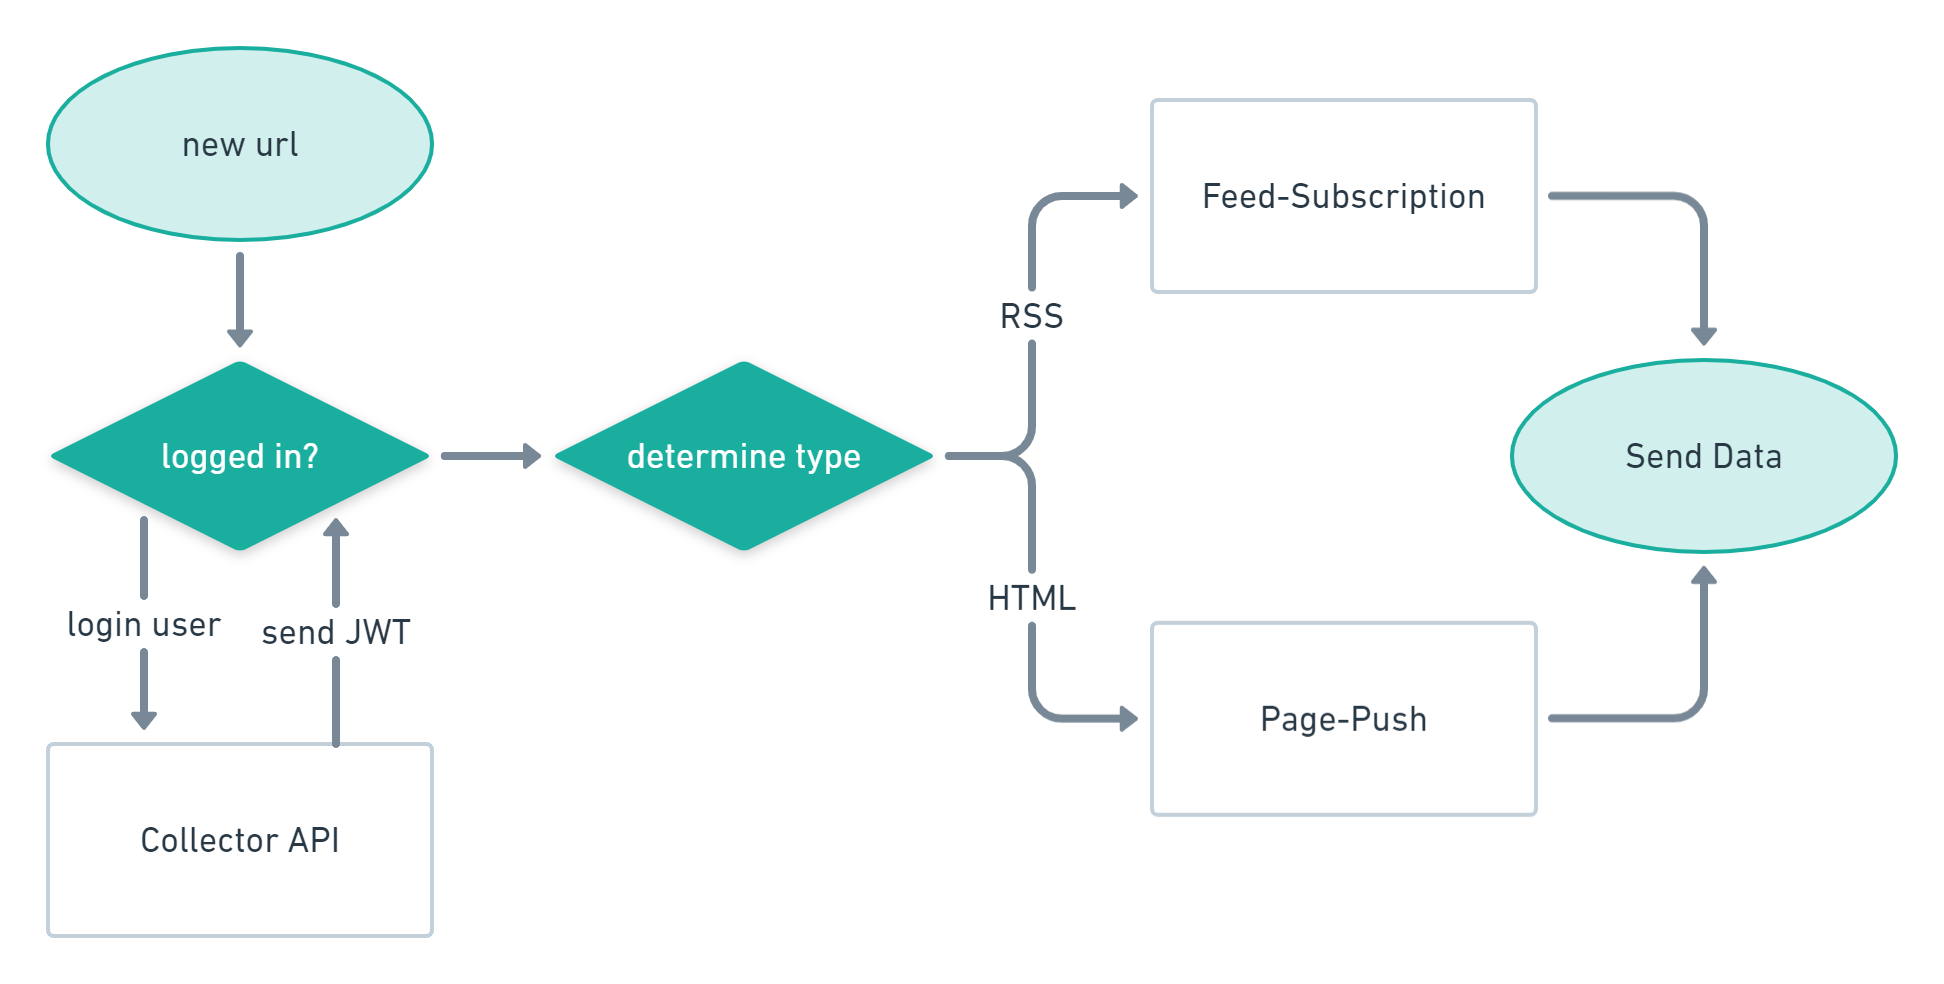
\includegraphics[width=\textwidth]{images/collector-pusher-process.png}
            \caption{Ablauf im Client-Pusher Systems}
        \end{center}
        
        \subsubsection{npm und die package.json}
            Im JavaScript Ökosystem wird der node package manager (npm) verwendet um Abhängigkeiten zu verwalten. Ähnlich Composer können Abhängigkeiten mittels \texttt{npm install} installiert werden und weitere Pakete mittels \texttt{npm install paketname} hinzugefügt werden. Informationen über die Abhängigkeiten werden in der \texttt{package.json} festgehalten, wo ebenfalls Scripts definiert werden können, welche für Build- und Compile-Prozesse verwendet werden.
            
            \begin{lstlisting}[caption=Ausschnitt package.json des Client-Pushers]
{
    "private": true,
    "scripts": {
    
        ...
        
        "prod": "npm run production"
        "production": "cross-env NODE_ENV=production node_modules/webpack/bin/webpack.js --no-progress --hide-modules --config=node_modules/laravel-mix/setup/webpack.config.js"
    },
   
    ...
    
    "dependencies": {
        "axios": "^0.18",
        "jquery": "^3.4.1",
        "normalize.css": "^8.0.1",
        "react": "^16.8.6",
        "react-dom": "^16.8.6",
        "select2": "^4.0.7",
        "sff": "^1.2.0"
    }
}
        \end{lstlisting}
        
        Im Client-Pusher wurde neben React folgende Pakete installiert:
        
        \begin{itemize}
            \item axios: Bibliothek um HTTP-Requests mit JavaScript zu vereinfachen
            \item jQuery: Bibilothek um den DOM vereinfacht zu manipulieren
            \item normalize.css: CSS-Dateien um browserspezifische Unterschiede vorzubeugen
            \item select2: Bibliothek zur verbesserten Darstellung von Select-Feldern
            \item sff: CSS-Framework zum beschleunigten Aufbau des User Interfaces
        \end{itemize}